%%%%%%%%%%%%%%%%%%%%%%%%%%%%%%%%%%%%%%%%%
% Journal Article
% LaTeX Template
% Version 2.0 (February 7, 2023)
%
% This template originates from:
% https://www.LaTeXTemplates.com
%
% Author:
% Vel (vel@latextemplates.com)
%
% License:
% CC BY-NC-SA 4.0 (https://creativecommons.org/licenses/by-nc-sa/4.0/)
%
% NOTE: The bibliography needs to be compiled using the biber engine.
%
%%%%%%%%%%%%%%%%%%%%%%%%%%%%%%%%%%%%%%%%%

%----------------------------------------------------------------------------------------
%	PACKAGES AND OTHER DOCUMENT CONFIGURATIONS
%----------------------------------------------------------------------------------------

\documentclass[
	a4paper, % Paper size, use either a4paper or letterpaper
	10pt, % Default font size, can also use 11pt or 12pt, although this is not recommended
	% unnumberedsections, % Comment to enable section numbering
	twoside, % Two side traditional mode where headers and footers change between odd and even pages, comment this option to make them fixed
]{journal}

\addbibresource{refs.bib} % BibLaTeX bibliography file

\runninghead{PHY324 Blackbody Radiation} % A shortened article title to appear in the running head, leave this command empty for no running head

\footertext{\textit{\today}} % Text to appear in the footer, leave this command empty for no footer tex

\setcounter{page}{1} % The page number of the first page, set this to a higher number if the article is to be part of an issue or larger work

%----------------------------------------------------------------------------------------
%	TITLE SECTION
%----------------------------------------------------------------------------------------

\title{\textcolor{bluehead}{Investigating Blackbody Emission Characteristics of a Tungsten Filament Light Bulb}} % Article title, use manual lines breaks (\\) to beautify the layout

% Authors are listed in a comma-separated list with superscript numbers indicating affiliations
% \thanks{} is used for any text that should be placed in a footnote on the first page, such as the corresponding author's email, journal acceptance dates, a copyright/license notice, keywords, etc
\author{%
    Julian Woo\thanks{julian.woo@mail.utoronto.ca}}
}
% Affiliations are output in the \date{} command
\date{\small PHY324 University of Toronto}

% Full-width abstract

%----------------------------------------------------------------------------------------
\newcommand{\roomTemp}{(22.20 \pm 0.05)^\circ \unit{C}}
\newcommand{\alphaNought}{(4.371 \pm 0.009)\cdot 10^{-3}\unit{K^{-1}}}
\newcommand{\thetainit}{(75.7 \pm 0.3)^\circ}
\renewcommand{\maketitlehookd}{%
	\begin{abstract}
        In this experiment, we tested how well an incandescent tungsten filament approximates a blackbody emitter by measuring its light spectrum over a range of temperatures. We used a prism-based spectrophotometer to record the bulb’s intensity distribution at different applied voltages and calculated filament temperatures from its electrical resistance. By fitting the peak wavelength of each measured spectrum, we confirmed that the peak emission shifts with temperature in a manner consistent with Wien’s Displacement Law, but we overestimate the Wien constant as $(3.8 \pm 0.3)\unit{m \cdot K}$. Our results also showed that the overall emission increases exponentially with temperature at a rate of $T^{4.62 \pm 0.02}$ in comparison with the $T^4$ dependence predicted by the Stefan-Boltzmann Law 
	\end{abstract}
}
\begin{document}

\maketitle % Output the title section




\section{Introduction}
\subsection{Physics of Blackbodies}
All objects with temperatures above absolute zero emit radiation as their thermal energy is converted into electromagnetic energy. By the reverse process, all objects also absorb electromagnetic radiation in a conversion to thermal energy. 

A blackbody is an idealized object in thermal equilibrium with its environment that absorbs all incoming radiation. To remain at the same temperature, the blackbody must necessarily emit radiation. The temperature of the blackbody, $T$, determines the intensity of this radiation. Planck's Law gives this intensity in a unit solid angle $d\Omega$ over some wavelength interval $d\lambda$, expressed as $I(\lambda, T)= dI/d\Omega d\lambda$. 
% \begin{equation}
% \label{eqn:planck_law}
%     I(\lambda, T ) = \frac{2hc^2}{\lambda^5}\frac1{e^{\frac{hc}{\lambda kT}} - 1}
% \end{equation}
% where $h$ is the planck constant, $k$ is the boltzmann constant. 
Figure \ref{fig:planck-law} illustrates how the intensity spectrum ($I(\lambda, T)$ across wavelengths) shifts with temperature, with the peak of the spectrum $\tub{\lambda}{max}$ given by Wien's Displacement Law, 
\begin{equation}
    \label{eqn:wein_displacement}
    \lambda_{\text{max}} T = 2.898 \times 10^{-3}\unit{m \cdot K}
\end{equation}

We can approximate real-world objects as blackbodies to study their thermal properties. As a body is heated, it will glow with a color closely characterized by the emission spectrum of a blackbody. Based on Figure \ref{fig:planck-law} and Wien's Displacement Law, higher temperatures correspond to lower peak wavelengths, explaining how bodies go from red-hot to white/blue-hot with increasing temperature. 

\begin{figure}[h]
    \centering
    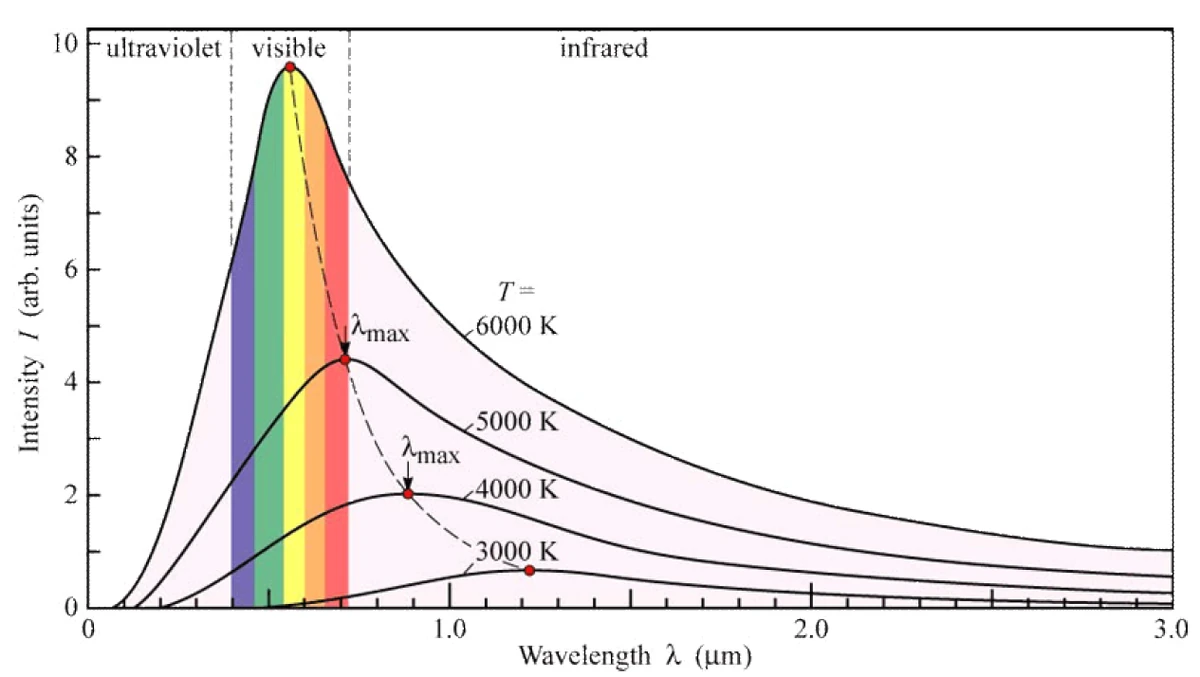
\includegraphics[width=\linewidth]{imgs/planck_law.png}
    \caption{Intensity spectra for an ideal blackbody as given by the Planck Law as function of wavelength at several temperatures. Taken from \autocite{Colose_2010}}
    \label{fig:planck-law}
\end{figure}
Experimentally, the total intensity of the radiation at the surface of a body, $I$, is related  to its temperature $T$ through the Stefan-Boltzmann Law
\begin{equation}
    \label{eqn:stefan-boltzmann-law}
    I = \epsilon \sigma T^4
\end{equation}
where $\epsilon$ is the emissivity of the surface ($\epsilon = 1$ for an ideal blackbody) and $\sigma = 5.67 \times 10^{-8} \text{ W} \cdot \text{m}^{-2} \cdot \text{K}^{-4}$ is the Stefan-Boltzmann constant.

In this experiment, we examine the emission spectrum of an incandescent tungsten filament light bulb across temperature to verify Wien's Displacement Law and the Stefan-Boltzmann Law. 

\subsection{Spectra via Diffraction}
To obtain the emission spectrum for a body, we can use a diffracting prism to separate the wavelengths of its emitted light over an angular spread and measure the intensity of the light across these angles. For a triangular prism with a 60$^\circ$ inner angle and back face perpendicular to the light beam as depicted Figure \ref{fig:prism_diagram}, Snell's law at the boundary where the ray enters and exits the prism yields 
\begin{align}
    \sin\theta_i &= n_p\sin\theta_2 \label{eqn:snell_incident}\\ 
    n_p\sin\theta_3 &= \sin \theta \label{eqn:snell_exit}
\end{align}
where $n_p$ is the index of refraction of the prism and the angles are defined as in Figure \ref{fig:prism_diagram}. The index of refraction of the surrounding air is taken to be 1. 

\begin{figure}[h]
    \centering
    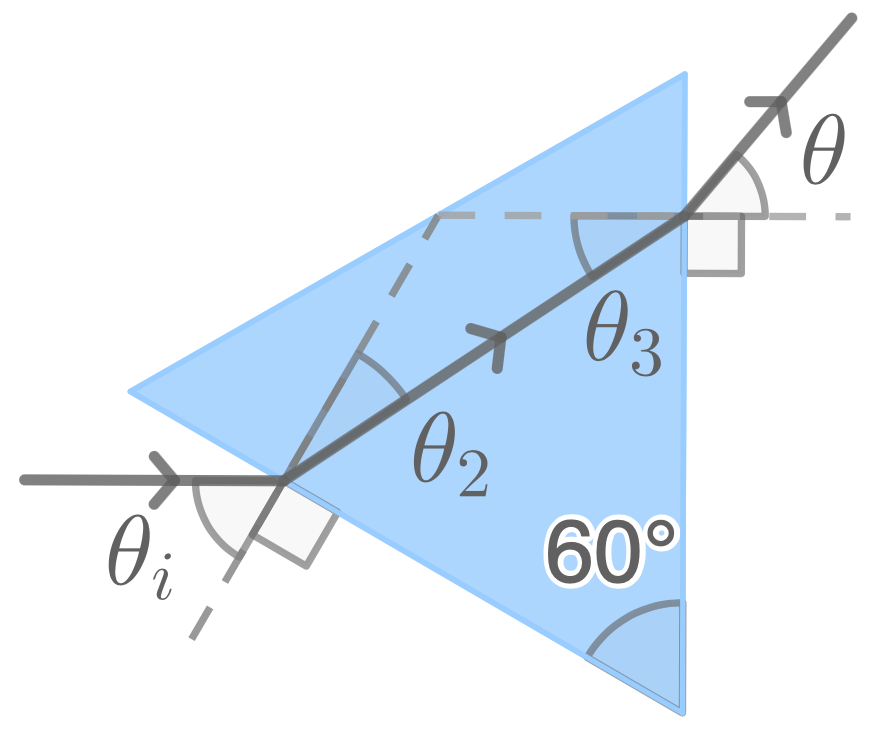
\includegraphics[width=0.6\linewidth]{imgs/prism_diagram.png}
    \caption{Diagram of path of light ray when diffracted in a triangular prism with $60^\circ$ inner angle and back face perpendicular to incident beam}
    \label{fig:prism_diagram}
\end{figure}


We are interested in the relationship between the exit angle $\theta$ and $n_p$. Equation \ref{eqn:snell_exit} provides $\sin \theta = n_p \sin \theta_3 = n_p \sin (60^\circ - \theta_2) =  n_p\frac{\sqrt3}{2}\sqrt{1 - \sin^2\theta_2} - \frac12 n_p\sin\theta_2$, where $\theta_2 + \theta_3 = 60^\circ$ is due to the prism geometry. Expressing $\sin\theta_2$ as $\sin \theta_i /n_p$ and simplifying provides 
\begin{equation}
    \label{eqn:np(theta, theta_i)}
    n_p(\theta, \theta_i) = \sqrt{\ab(\frac{2\sin\theta + \sin\theta_i}{\sqrt3})^2 + \sin^2\theta_i}
\end{equation}
For an incidence angle of $\theta_i = 60^\circ$, this reduces to 
\begin{equation}
    \label{eqn:np(theta)}
    n_p(\theta) = \sqrt{\ab(\frac2{\sqrt3}\sin \theta + \frac12)^2 + \frac34}
\end{equation}
We relate the index of refraction to the wavelength of light through the Cauchy equation suppressed to two-terms 
\begin{equation}
    \label{eqn:cauchy}
    n_p(\lambda) = \frac{A}{\lambda^2} + B
\end{equation}
where $A$ and $B$ depend on the material of the prism. Composing these two relations gives the wavelength of the light in terms of its exit angle
\begin{equation}
\label{eqn:lambda(theta)}
    \lambda(\theta) = \sqrt{\frac{A}{n_p(\theta) - B}}
\end{equation}
Figure \ref{fig:lambda_hmap} demonstrates the dependence of $\lambda$ on the exit angle around an incidence angle of 60$^\circ$ for set Cauchy parameters. The wavelengths fall off steeply from the singularity at $n_p = B$, going from 3500nm to 1500nm within less than half a degree increase in either the incidence or exit angle.

Prisms do not diffract all incoming light. Some light is able to pass through un-deflected. Based on Figure \ref{fig:prism_diagram}, this introduces a second smaller peak in the emission spectra of the body (see Figure \ref{fig:planck-law}) at $\lambda(\theta = 0)$, provided the detector is far enough away from the prism.
\begin{figure}[h]
    \centering
    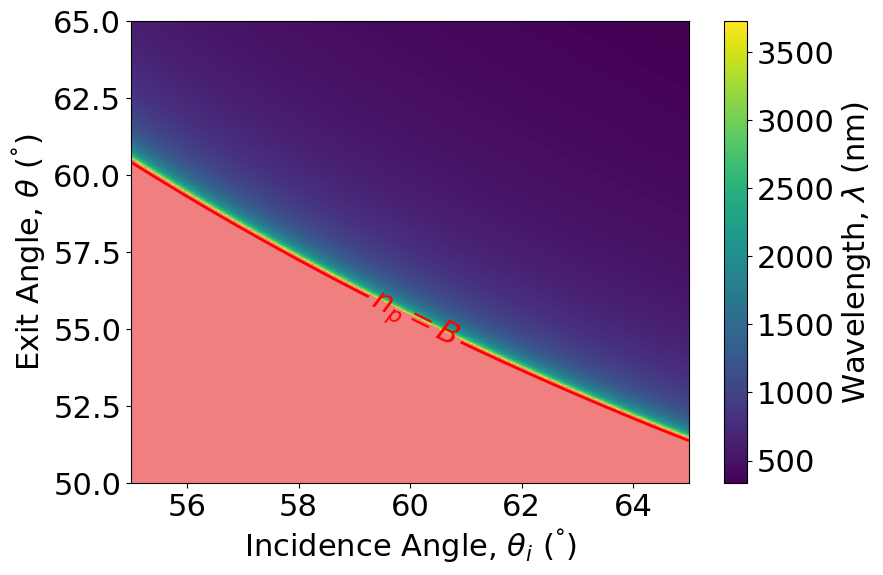
\includegraphics[width=\linewidth]{imgs/lambda_hmap.png}
    \caption{Theoretical wavelength of light diffracted via triangular prism shown in Figure \ref{fig:prism_diagram} as function of incident angle $\theta_i \in [55^\circ, 65^\circ]$ and exit angle $\theta \in [50^\circ, 65^\circ]$. Heatmap values generated by Equation \ref{eqn:lambda(theta)} with $A = 13900\unit{nm^2}$ and $B = 1.689$. Limited to $n_p \geq B + 0.001$ to avoid singularity. Red contour line indicates $n_p = B$ and light-red region corresponds to $n_p < B$.}
    \label{fig:lambda_hmap}
\end{figure}


\subsection{Resistance and Temperature}
We can determine the temperature of the material under study using resistance measurements. For small enough changes, the resistance, $R$, of a conducting material can be expanded to first order around some temperature $T_0$ as 
\begin{equation}
    \label{eqn:R(T)_firstorder}
    R(T) = R(T_0)[1 + \alpha_0(T - T_0)]
\end{equation}
where $\alpha_0$ is temperature coefficient of the material at $T_0$. If an analytical form for $R(T)$ is known, $\alpha_0$ can be determined as 
\begin{equation}
    \label{eqn:alpha0}
    \alpha_0 = \frac{R'(T_0)}{R(T_0)}
\end{equation}
This expression also holds for the resistivity of the material, since it is related to resistance by some geometric factor. 

If a DC voltage, $V$, is applied through the material to generate a current $I$, we will have $V = IR(T)$. Rearranging for temperature, we find 
\begin{equation}
    \label{eqn:T(V,I)}
    T = T_0 + \frac{\frac{V}{IR(T_0)} - 1}{\alpha_0}
\end{equation}
For tungsten filament, we take $R(T_0) = 1.1\Omega$ \autocite{bbody324labmanual}. Thus, if we know the voltage and current through a material, we can determine its temperature, provided its coefficient is known. 

\section{Methods and Procedures}
A prism-based PASCO OS-8537 spectrophotometer, as shown in Figure \ref{fig:expsetup}, was used to examine the spectrum of light emitted by a tungsten-filament light bulb at different temperatures. The light from the bulb is collimated by a lens approximately 10cm away to make the light rays parallel to prevent convergence or divergence. This beam is shone on a diffracting prism with an internal angle of $60^\circ$ and its back face perpendicular to the beam, as diagrammed in Figure \ref{fig:prism_diagram}. According to \cite{bbody324labmanual}, the prism is characterized by Cauchy parameters $A = 13900\unit{nm^2}$ and $B = 1.689$ in Equation \ref{eqn:cauchy}. The setup is calibrated such that the incidence angle of the beam is 60$^\circ$ so that Equation \ref{eqn:np(theta)} holds. The intensity of the diffracted light is recorded by a PASCO CI-6630 broad spectrum light sensor on an arm which can rotate in 90$^\circ$ or $30^\circ$ arcs from its starting position. A mask with variable slit sizes is attached to the front of the light sensor to diminish stray light effects. We use slit \#4 throughout the experiments. The light sensor additionally has 3 selectable gains of 1, 10 and 100.  

A computer data acquisition system with proprietary UofT labview software is used to source a voltage to the bulb through a CI-6552A Power Amplifier and record the bulb current with empirical uncertainty of $0.005\unit{A}$. The system permits bulb voltages within 4$\unit{V}$ to 10$\unit{V}$. With a bulb voltage selected, the light sensor is rotated from its starting position and the system records and displays intensity readings (converted to voltages) at the angular position determined by the internal CI-6538 rotary motion sensor. Data collection and voltage sourcing is automatically halted when the light sensor arm hits its stopping point. All data was collected in a room with the lights turned off, however, ambient light from computer screens and various indicator lights persisted. 

We carried out 2 experiments to verify Wien's displacement Law and the Stefan Boltzman Law separately.

\begin{figure}[h]
    \centering
    \includegraphics[width=\linewidth]{imgs/bb_expsetup.png}
    \caption{Experimental Setup. Incandescent tungsten filament light bulb (far left) aligned with diffracting prism and intensity recorded by light sensor on rotating arm (far right)}
    \label{fig:expsetup}
\end{figure}

\subsection{Wien Experiment Procedure}
The bulb voltage was set to 4V and the light sensor gain to 100. Setting the scan size to 90 degrees, the sensor arm was rotated slowly by hand until data collection halted. 5 sets of data were taken in this manner.

The bulb voltage was then varied from $4\unit{V}$ to $10\unit{V}$ in $0.5\unit{V}$ increments with the light sensor gain set to 100 for voltages below $6\unit{V}$ and 10 beyond. The sensor was tared when the gain was altered to remove biases. At each bulb voltage, a $30^\circ$ scan was performed from the starting position, with the sensor rotated slower through the peak region of the intensity spectrum to sample more points. We export the intensity and angle data for each scan and combine it with the bulb voltage and bulb current values to create another dataset.

\subsection{Stefan-Boltzmann Experiment Procedure}
We again vary the bulb voltage from $4\unit{V}$ to $10\unit{V}$ in $0.5\unit{V}$ increments with the sensor gain set to a constant 10. For each bulb voltage, 3 $30^\circ$ scans are taken after setting the sensor to its starting position and rotating it slower within the peak region. Beyond $9\unit{V}$, the displayed spectra were observed to plateau near the top of the peak, possibly due to reaching voltage limits of the light sensor. The bulb voltage and bulb current readings were combined with the intensity and angle data from the scans to create a third dataset.

Lastly, the temperature of the room was measured with a Digital Infrared Thermometer pointed to one of the walls.
\section{Analysis and Discussion}
We seek to corroborate Wien's Displacement Law and the Stefan-Boltzmann Law by examining the intensity spectrum of an incandescent tungsten filament light bulb using a prism spectrophotometer as the bulb voltage is varied within the range $4\unit{V}$ to $10\unit{V}$. The color from the bulb was observed to go from a warm amber to a bright yellow with increasing bulb voltage. Further, the diffracted light was seen to produce a rainbow on the light sensor mask with colors ranging from blue to red. The ambient temperature of the room was determined to be $T_R = \roomTemp$. White and Minges provide a 4th-order fit for the resistivity of tungsten in the range 100K to 3600K given by $\rho(T) = \sum_{n = 0}^4A_n(T/1000)^n$ achieving an rms deviation of 0.2\% \autocite{White_Minges_1997}. The $A_n$ coefficients are given in the appendix. From this, we determine $\alpha_0(T_R)$ using equation \ref{eqn:alpha0} with $\rho$ in place of $R$ to get $\alpha_0(T_R) = \alphaNought$. Calculation details are provided in Appendix Section \ref{appendix:white-minges-fit-parameters}.  With this, the bulb voltage and bulb current readings are converted to bulb temperatures using equation \ref{eqn:T(V,I)}. The bulb temperature was found to increase with bulb voltage, going from $(2380 \pm 30)\unit{K}$ at 4V to $(3520 \pm 30)\unit{K}$ at 10V.

\subsection{Wien Experiment Analysis}
By averaging the locations of the secondary peaks in the calibration dataset of 5 90 degree scans we determine the sensor position $\theta_0$ corresponding to an exit angle of 0 for the diffracted light. We find $\theta_{0} = \thetainit$. The remaining 30 degree scans as the bulb voltage is varied are used to determine the peak wavelength of the spectrum as a function of temperature. The gains during these scans varied from 10 to 100, but this only alters the magnitude of the intensities, with the peaks ideally remaining in the same locations for each voltage. Wavelengths are obtained through equation \ref{eqn:lambda(theta)} with the exit angle $\theta$ given the angle difference between the peaks and $\theta_0$. Of the 13 scans, two produced $n_p(\theta) < B$ which correspond to unphysical wavelengths. Uncertainties in these wavelengths are estimated by propagating the uncertainty in $\theta_0$ through Equation \ref{eqn:lambda(theta)} as shown in Appendix Section \ref{appendix:wavelength-uncertainty-prop}. The data at $4, 4.5, 8$ and $10$ volts produced larger wavelengths leading to uncertainties greater than the wavelengths themselves due to the $\lambda^3$ dependence in the formula \ref{eqn:dlambda_dtheta}. These points are discarded in the analysis. 

We also generate intensity spectra of the bulb at various temperatures (see Figure \ref{fig:wein_q3} in \nameref{appendix:supp-figs}) to observe their behavior. To do so, the intensity readings are bias-subtracted, with the bias taken to be the intensity at the smallest angular position. The spectrum is then normalized by multiplying the intensity readings by $1/I^*$ where $I^*$ is the maximum intensity reading. 

\begin{figure}[h]
    \centering
    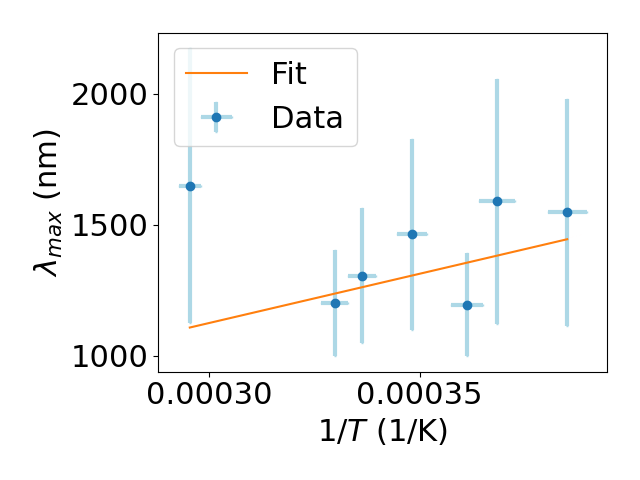
\includegraphics[width=0.8\linewidth]{imgs/wein_lambda_invT.png}
    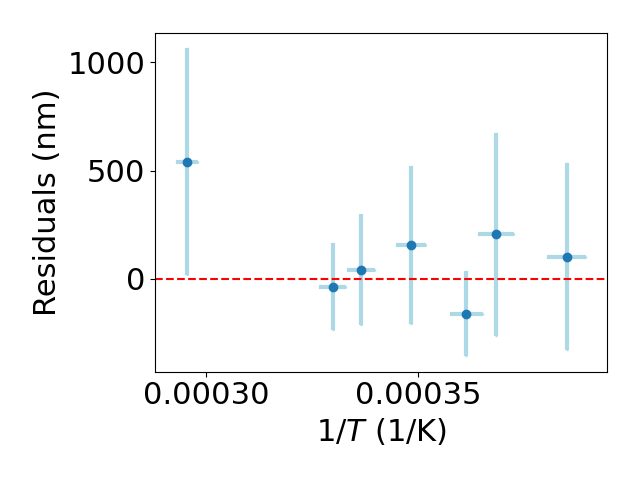
\includegraphics[width=0.8\linewidth]{imgs/wein_lambda_invT_res.png}
    \caption{(Top) Peak wavelengths of intensity spectrum of tungsten filament light bulb plotted against inverse of bulb temperature. Proportional fit with constant $(3.8 \pm 0.3)\unit{m \cdot K}$ achieves $\chi_{red} = 0.4$ and $\chi_{prob} = 0.9$. (Bottom) Residuals of fit}
    \label{fig:wein_lambda_invT}
\end{figure}

We fit a linear function to the peak wavelength against inverse bulb temperature which should be proportionally related by the Wien constant from Wien's Displacement Law (Equation \ref{eqn:wein_displacement}). The fit is shown in Figure \ref{fig:wein_lambda_invT} to give a Wien constant of $(3.8 \pm 0.3)\cdot 10^{-2}\unit{m \cdot K}$ overestimating the true value by an order of magnitude. The relative error on the wavelengths approach 30\%, so the  decent goodness of fit statistics are likely inflated. The residuals appear patternless, although they may not be manifest with our sample of 7 points. Figure \ref{fig:wein_lambda_invT} demonstrates that the peak wavelength generally increases with lower temperatures with a noticeable outlier at $0.00030\unit{K^{-1}}$. The errorbar for this datapoint is also exaggerated given it produced a larger wavelength value and our uncertainties scale with $\lambda^3$ (see Appendix Section \ref{appendix:wavelength-uncertainty-prop}). Overall, the trend in Figure \ref{fig:wein_lambda_invT} supports the observation of our bulb color going from amber to bright yellow with higher voltages. These voltages correspond to higher temperatures which are met with lower wavelengths and thus lighter color. Figure \ref{fig:wein_q3} shows how our intensity spectra shift with temperature. We see that at higher temperatures, the spectrum generally shifts to include more wavelengths in the visible spectrum. Thus, the bulb can be made to radiate more visible light by increasing its temperature.  

The large uncertainties in our wavelengths can be traced back to our determination of $\theta_0$, the sensor position when incident with the un-deflected light beam. A higher precision measurement of this value would greatly benefit the analysis. A motorized arm could be used to slowly sweep the detector instead of by hand. This would allow for finer sampling of the sensor angular position, which would then improve the resolution of the peak locations at both the main and secondary peak. Beyond that, we were unable to verify the alignment of the prism. Figure \ref{fig:lambda_hmap} demonstrates the sensitivity of the system to small changes in the incidence and exit angle of the beam. It is possible that our incidence angle was slightly lower than $60^\circ$, pushing us closer to the contour where $n_p = B$ which led us to produce 2 unphysical data points with $n_p < B$. This would lead to inflated wavelengths due to Equation \ref{eqn:lambda(theta)}, which in turn generate larger uncertainties through Equation \ref{eqn:dlambda_dtheta}. Hence, future experiments should focus efforts to verifying prism alignments.

Since the tungsten filament light bulb only approximates an ideal blackbody, we would expect that its intensity is lower than predicted by the Planck Law as it will reflect incoming radiation. However, if this reflection is uniform across wavelengths, the peak should still occur at the same wavelength, so Wien's Displacement Law should still hold. Hence, it is likely that our experimental errors have larger influence on our findings. If needed, the filament could be replaced by a insulated enclosure with a small cavity to better approximate a blackbody. 

\subsection{Stefan-Boltzmann Analysis}
The total intensity from the light source is proportional to the integral of the intensity readings from the light sensor over the peak region. To generate these integrals, the labview software was used during data collection with cursors placed approximately $\pm 10^\circ$ from the peak to remove baseline effects. The bulb voltages and currents are converted to temperatures in the same manner as before. Two data points at voltages of 9.5V and 10V were determined to be outliers as they generated intensity integrals lower than the general trend suggested. This is likely due to the clipping of the spectrum observed during data collection. With these removed, we fit a functional form of $AT^x$, with the fit parameter $x$ expected to be 4 as in the Stefan-Boltzmann Equation \ref{eqn:stefan-boltzmann-law}. 

Figure \ref{fig:stef_powfit} provides the fit for our intensity and temperature data, yielding an exponent of $4.62 \pm 0.02$ with reasonable goodness of fit and patternless residuals. The exponent is higher than expected, indicating that our intensities are increasing at higher rate, or we are underestimating our bulb temperatures. 

The ambient light in the room, if constant throughout data collection, would contribute a global shift in the intensity spectra we collect that may not be accounted for when restricting the integral to the peak region. This would additionally lead to higher internsity readings causing our power law fit to overestimate the Stefan-Boltzmann constant. This could be countered by including a vertical shift in the fitting function, however, when this was attempted, we found the quality of the fit decreased significantly. Future experiments would benefit from collecting data in a certified dark room to minimize ambient light effects. Further, the ambient light was not constant with doors being opened and closed letting more light in during some scans than others. Outside of outlier points, this would contribute noise to the intensity readings.



\begin{figure}[h]
    \centering
    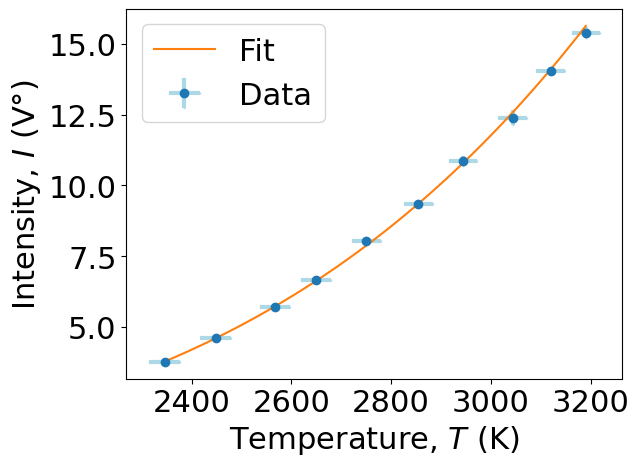
\includegraphics[width=0.8\linewidth]{imgs/stef_powfit.png}
    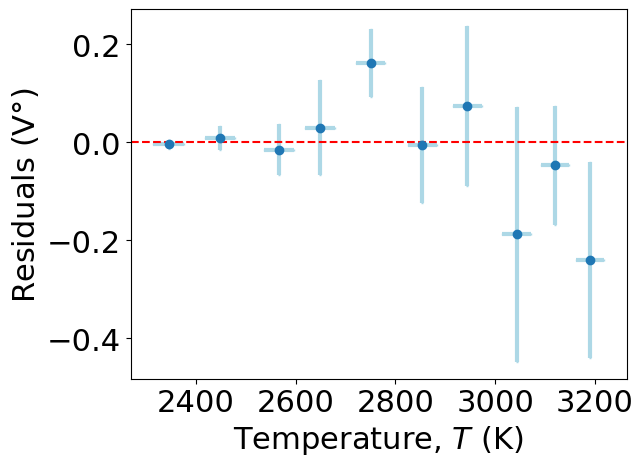
\includegraphics[width=0.8\linewidth]{imgs/stef_powfit_res.png}
    \caption{(TTop) Integral of intensity spectrum of tungsten filament light bulb recorded in voltages over angular position plotted against bulb temperature. Power law fit of $AT^x$ with  $A = (1.0 \pm 0.1)\unit{V^\circ K^{-x}}$ and $x = (4.62 \pm 0.02)$ achieves $\chi_{red} = 1.0$ and $\chi_{prob} = 0.41$. (Bottom) Residuals of fit}
    \label{fig:stef_powfit}
\end{figure}


\section{Conclusion}
In this experiment, we used an incandescent tungsten filament light bulb to examine its approximate blackbody behaviour over a range of temperatures. Our primary aim was to verify Wien’s Displacement Law by tracking how the peak emission wavelength shifts as the filament temperature changes, and we also assessed whether the overall intensity follows the Stefan–Boltzmann relationship. To do this, we varied the applied voltage, measured the electrical resistance to estimate temperature, and recorded the emission spectrum using a prism-based spectrophotometer. By fitting the peak wavelength of each  measured spectrum, we confirmed that the emission shifts with temperature in a manner consistent with Wien's Displacement Law. However, we overestimated the Wien constant as $(3.8 \pm 0.3)~\mathrm{m\cdot K}$ when compared to the literature value $2.898 \times 10^{-3}\unit{m \cdot K}$. Moreover, our results showed that the overall light intensity increases with temperature following a power law of $T^{4.62 \pm 0.02}$, in comparison with the $T^{4}$ dependence predicted by the Stefan-Boltzmann Law  Despite some limitations, such as incomplete wavelength coverage and the need for more precise spectrometer calibration, our results affirm the tungsten filament’s close conformity to blackbody behavior.




%	 REFERENCES
%----------------------------------------------------------------------------------------

\printbibliography % Output the bibliography


%----------------------------------------------------------------------------------------

\newpage

\appendix
\section*{Appendix}
\renewcommand{\thesubsection}{\Roman{subsection}}
\textbf{Statement of AI Usage} Used Vscode automatic code suggestions from Github Copilot and Coedeium during analysis to help write out functions and debug. 

\subsection{Wavelength Uncertainty Propagation}
\label{appendix:wavelength-uncertainty-prop}
To determine the uncertainty in wavelength, $u(\lambda)$, we propagate equation \ref{eqn:lambda(theta)}, using experimental uncertainties for $\theta$ to get 
\begin{equation}
    u(\lambda) = \ab|\diffp{\lambda}{\theta} u(\theta)|
\end{equation}
We have 
\begin{align*}
    \diffp{\lambda}{n}
    &= \frac12\ab(\frac{A}{n - B})^{-1/2} \frac{-A}{(n - B)^2} = \frac{-\lambda^4}{2A\lambda} = -\frac{\lambda^3}{2A}
\end{align*}
and 
\begin{align*}
    \diffp{n}{\theta}
    &= \frac1{2n}\cdot 2\ab(\frac2{\sqrt3}\sin\theta + \frac12)\cdot \frac2{\sqrt3}\cos\theta \\ 
    &= \frac{2\cos\theta\sqrt{n^2 - \frac34}}{n\sqrt 3}
\end{align*}
Together, we get 
\begin{align}
\label{eqn:dlambda_dtheta}
    \diffp{\lambda}{\theta} &= \diffp{\lambda}{n} \diffp{n}{\theta} = \frac{-\lambda^3\cos\theta\sqrt{n^2 - \frac34}}{nA\sqrt 3}
\end{align}

\subsection{White Minges Fit Parameters}
\label{appendix:white-minges-fit-parameters}
White and Minges fit the resistivity of Tungsten in the range 100K to 3600K using a 4th order polynomial $\rho(T) = \sum_{n = 0}^4A_n(T/1000)^n$ with coefficients given by Table \ref{tab:white_minges_fit_cieffs}

\begin{table}[h]
\centering
\caption{Coefficients for a 4th order fit of the electrical resistivity of tungsten by White and Minges \autocite{White_Minges_1997} in the range 100$\unit{K}$ to 3600$\unit{K}$ given by $\rho(T) = \sum_{n = 0}^4A_n(T/1000)^n$}
\label{tab:white_minges_fit_cieffs}
\resizebox{0.45\columnwidth}{!}{%
\begin{tabular}{@{}ll@{}}
\toprule
$n$ & $A_n$ ($\unit{10^{-8} \Omega \cdot m \cdot K^{-n}}$) \\ \midrule
0   & -0.968                                               \\
1   & 19.724                                               \\
2   & 7.826                                                \\
3   & -1.8517                                              \\
4   & 0.2079                                               \\ \bottomrule
\end{tabular}%
}
\end{table}
The temperature coefficient of tungsten at some $T_0$ is determined via equation \ref{eqn:alpha0} with $\rho$ in place of $R$ to give 
\begin{align*}
    \alpha_0(T_0) = \frac{\sum_{n = 0}^4 nA_n T_0^{n- 1}/1000^n}{\sum_{n = 0}^4A_n(T_0/1000)^n}
\end{align*}
For $T_R = \roomTemp$, we get 
\begin{equation}
\alpha_0(T_R) = (4.371 \pm 0.009)\unit{K^{-1}}
\end{equation}
where the relative uncertainty is taken to be 2\% to match the rms deviation in the White and Minges fit \autocite{White_Minges_1997} which dominates compared to the 0.2\% error in the temperature reading obtained by the Digital Infrared Thermometer.

\subsection{Supplementary Figures}
\label{appendix:supp-figs}
\begin{figure}[h]
    \centering
    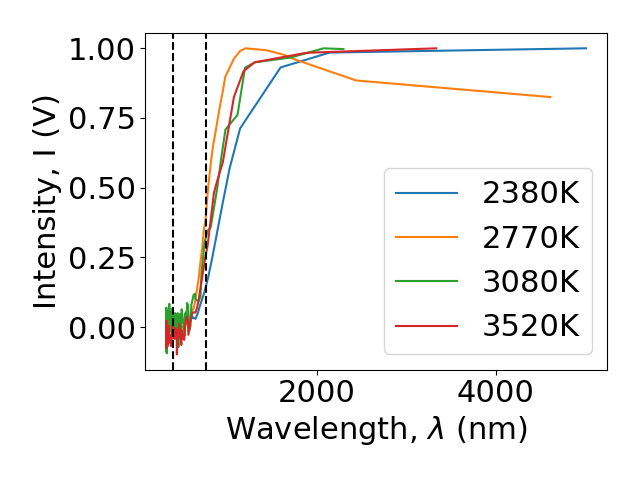
\includegraphics[width=0.9\linewidth]{imgs/wein_q3.png}
    \caption{Normalized, bias-subtracted Intensity spectra of Tungsten Filament Light Bulb at various bulb Temperatures. Bulb Temperatures are $\pm 30\unit{K}$. Vertical lines at 380$\unit{nm}$ and 750$\unit{nm}$ indicate boundaries of visible spectrum.}
    \label{fig:wein_q3}
\end{figure}



\end{document}
